\section{Resuelva el siguiente p.p.l por el método simplex, comenzando con la
solución básica factible $(x_1, x_2) = (4,0)$.}
\begin{tabular}{|l|l|}
\hline
Max  & -x_1+2x_2        \\ \hline
s.a. & 3x_1+4x_2=12     \\ \hline
     & 2x_1-x_2 \leq 12 \\ \hline
     & x_1,x_2 \geq 0   \\ \hline
\end{tabular}
$$\Rightarrow x=\begin{pmatrix}x_1\\ x_2\\ x_3\end{pmatrix}=\begin{pmatrix}0\\ 0\\ 12\end{pmatrix}, z=0 \mbox{  Punto $(0,0 )$}$$

ahora para el punto dado tenemos:

\begin{tabular}{|l|l|l|l|l|l|}
\hline
Tabla 2 &   &     & -1  & 2    & 0   \\ \hline
Base    & z & x_0 & x_1 & x_2  & x_3 \\ \hline
x_1     & 0 & 0   & 1   & -2   & 0   \\ \hline
z       & 1 & 4   & 1   & 1.35 & 0   \\ \hline
\end{tabular}
\Rightarrow
\begin{tabular}{|l|l|l|l|l|l|}
\hline
Tabla 3 &   &     & -1   & 2   & 0   \\ \hline
Base    & z & x_0 & x_1  & x_2 & x_3 \\ \hline
x_2     & 0 & 3   & 2.5  & 0   & 0   \\ \hline
z       & 1 & 6   & 0.75 & 1   & 0   \\ \hline
\end{tabular}

$$\Rightarrow x=\begin{pmatrix}0\\ 3\\ 0\end{pmatrix},\: z=6 \mbox{ Punto } (0,3)$$

\section*{Grafique la región factible en el espacio de las variables no-básicas.}

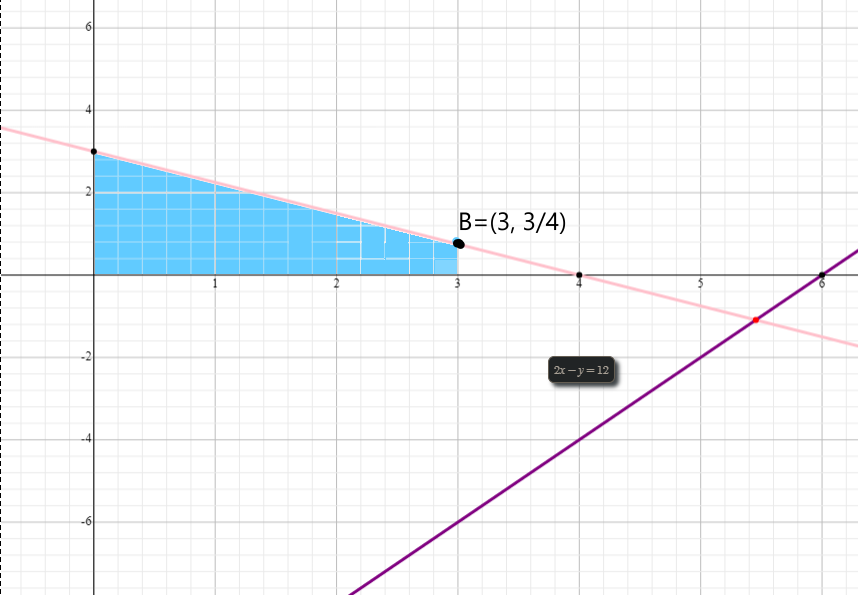
\includegraphics[scale=0.2]{Ejercicios/graficas/Ejercicio4.png}